\documentclass{article}

\usepackage{graphicx}
\usepackage{tikz}
\usepackage{tikzsymbols}
\usetikzlibrary{calc,patterns,shapes.geometric}
\pagestyle{empty}
\usepackage[margin=0pt]{geometry}
\geometry{papersize={14in,12in}}

\def\centerarc[#1](#2)(#3:#4:#5){\draw[#1] ($(#2)+({#5*cos(#3)},{#5*sin(#3)})$) arc (#3:#4:#5);}

\begin{document}
	\begin{figure}
		\centering
		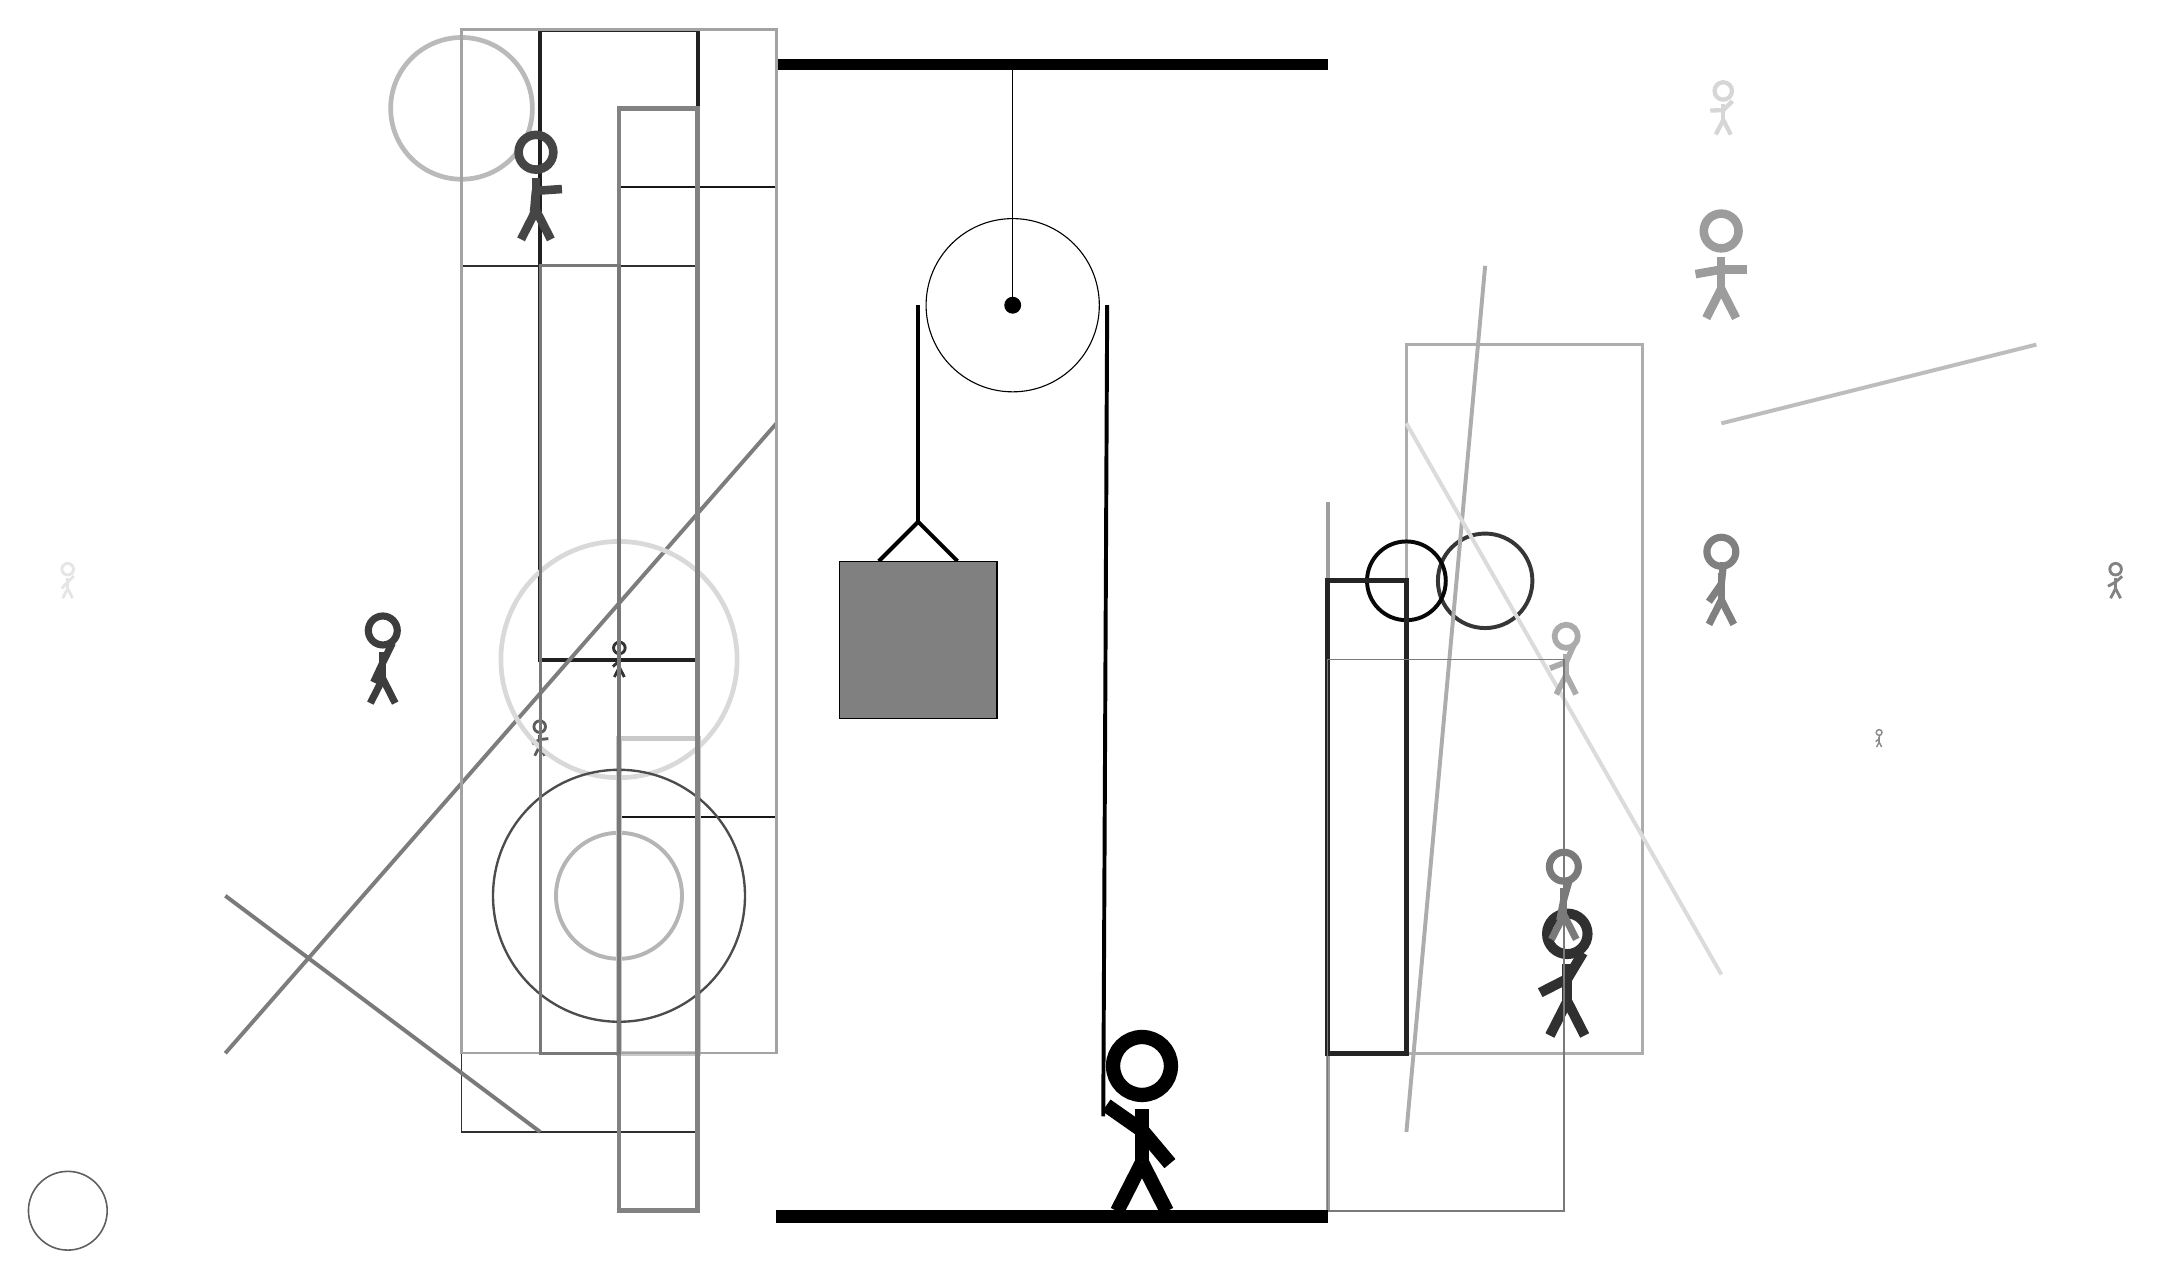
\begin{tikzpicture}
			%%%%% START %%%%%
			
			\draw[fill=black] (-2, 11.5) rectangle (5, 11.625);
			
			\draw[line width=0.5mm, color=black!28](5, 3) -- (5, -2);
			
			\draw [line width=0.5mm, color=black!29](-4, 1) circle (0.8);
			\node[line width=0.7mm, color=black!16] at (10, 11) {\Strichmaxerl[3][1][45]};
			\draw[line width=0.5mm, color=black!87] (-3, 4) rectangle (-5, 12);
			
			\node[line width=0.4mm, color=black!80] at (-4, 4) {\Strichmaxerl[2][42][87]};
			\node[line width=0.5mm, color=black!49] at (15, 5) {\Strichmaxerl[2][29][41]};
			\draw[line width=0.5mm, color=black!38] (5, 6) rectangle (5, -3);
			\draw[line width=0.5mm, color=black!26](10, 7) -- (14, 8);
			\node[line width=0.5mm, color=black!50] at (10, 5) {\Strichmaxerl[5][55][84]};
			\draw [line width=0.5mm, color=black!79](7, 5) circle (0.6);
			\node[line width=0.6mm, color=black!64] at (-5, 3) {\Strichmaxerl[2][30][6]};
			\node[line width=0.7mm, color=black!81] at (8, 0) {\Strichmaxerl[7][27][59]};
			\node[line width=0.6mm, color=black!52] at (8, 1) {\Strichmaxerl[5][79][74]};
			\draw[line width=0.5mm, color=black!32](7, 9) -- (6, -2);
			\draw [line width=0.6mm, color=black!27](-6, 11) circle (0.9);
			\node[line width=0.7mm, color=black!39] at (10, 9) {\Strichmaxerl[6][10][0]};
			\draw[line width=0.5mm, color=black!51](-2, 7) -- (-9, -1);
			\node[line width=0.5mm, color=black!46] at (12, 3) {\Strichmaxerl[1][37][84]};
			\draw [line width=0.2mm, color=black!63](-11, -3) circle (0.5);
			\draw[line width=0.4mm, color=black!32] (6, 8) rectangle (9, -1);
			\draw [line width=0.5mm, color=black!97](6, 5) circle (0.5);
			\draw[line width=0.2mm, color=black!81] (-3, -2) rectangle (-6, 9);
			\draw [line width=0.6mm, color=black!15](-4, 4) circle (1.5);
			\draw[line width=0.3mm, color=black!91] (-2, 2) rectangle (-4, 10);
			\node[line width=0.4mm, color=black!76] at (-7, 4) {\Strichmaxerl[5][65][64]};
			\draw[line width=0.7mm, color=black!21] (-3, 3) rectangle (-4, -1);
			
			\draw[line width=0.3mm, color=black!36] (-2, -1) rectangle (-6, 12);
			\node[line width=0.4mm, color=black!73] at (-5, 10) {\Strichmaxerl[6][85][4]};
			
			\draw[line width=0.5mm, color=black!14](6, 7) -- (10, 0);
			\draw[line width=0.6mm, color=black!86] (6, -1) rectangle (5, 5);
			\draw [line width=0.3mm, color=black!70](-4, 1) circle (1.6);
			\node[line width=0.5mm, color=black!33] at (8, 4) {\Strichmaxerl[4][21][66]};
			\draw[line width=0.6mm, color=black!49] (-3, -3) rectangle (-4, 11);
			
			\draw[line width=0.4mm, color=black!53] (-4, 9) rectangle (-5, -1);
			\draw[line width=0.2mm, color=black!52] (5, 4) rectangle (8, -3);
			\draw[line width=0.5mm, color=black!52](-5, -2) -- (-9, 1);
			\node[line width=0.3mm, color=black!10] at (-11, 5) {\Strichmaxerl[2][47][44]};
			
			\draw (1, 8.5) circle (1.1);
			\draw[fill=black] (1, 8.5) circle (0.1);
			\draw (1, 11.5) -- (1, 8.5);
			
			\draw[line width=0.5mm] (-0.7, 5.25) -- (-0.2, 5.75) -- (0.3, 5.25);
			\draw[fill=black!50] (-1.2, 5.25) rectangle (0.8, 3.25);
			
			\draw[line width=0.5mm] (-0.2, 8.5) -- (-0.2, 5.75);
			\centerarc[line width=0.5mm](1, 8.5)(0:180:1.2000000000000002);
			\draw[line width=0.5mm](2.2, 8.5) -- (2.15, -1.8);
			
			\node at (2.6, -1.9) {\Strichmaxerl[10][-35][-50]};
			
			\draw[fill=black] (-2, -3) rectangle (5, -3.15);
			
			%%%%% END %%%%%
		\end{tikzpicture}
	\end{figure}	
\end{document}